\section{Extensions}

\textbf{Dynamic Re-routing}\\
The real tourist behavior and weather conditions, are dynamic and unpredictable in nature. They can be influenced by unforeseen delays, detours, longer-than-anticipated visits, or spontaneous user preferences, which can significantly impact the feasibility and correctness of an advanced preplanned itinerary. To close the gap between theory and practice, a dynamic approach is required.

In contrast with the static approach used in \cite{taylor2018tour}, where rigid, precomputed travel times and POI visit times, we have taken real-time travel times using Google-Maps API (Routes API). 

On the top of suggested times of visit and travel, user can enter the actual time they have taken to visit a POI and the travel time they took to reach the current POI.

With every visit to a POI, the system replans the schedule based on the remaining time and cost budgets. The POIs already visited are not considered for further itineraries. This optimizes the rest of the day based on current progress and not stale assumptions.

For the dynamic feature, a record of visited POIs was maintained. On visiting a POI, it was eliminated from the list to be taken into account in future itinerary calculations with the new remaining time and cost budgets.

\begin{figure}[H]
\textbf{Implementation of Dynamic Approach}
\centering
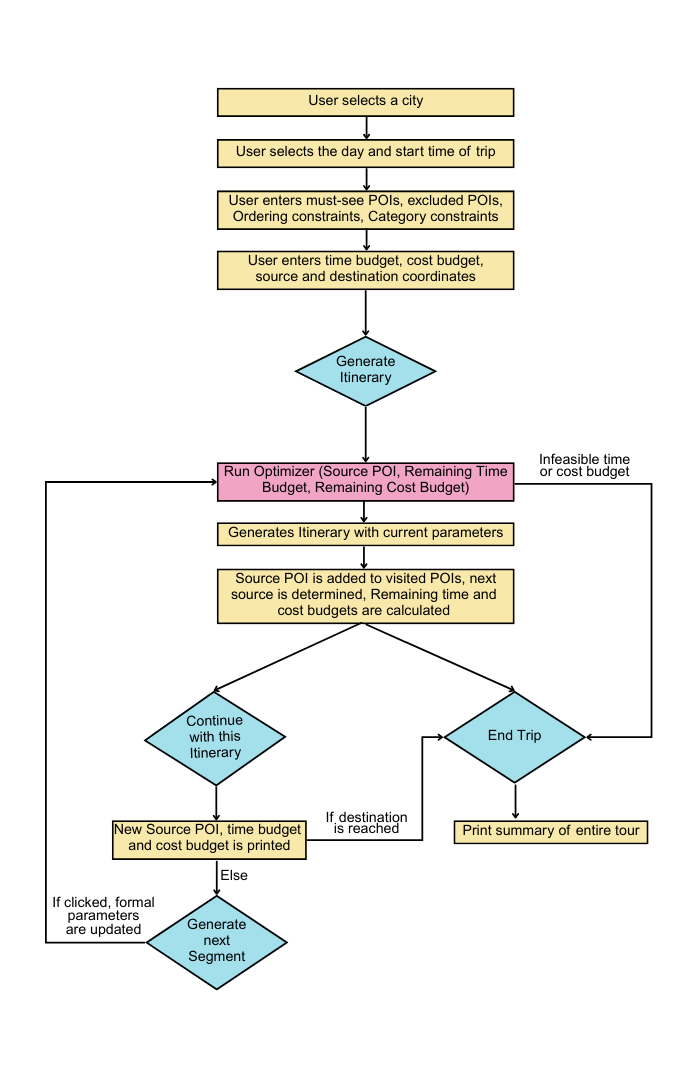
\includegraphics[width=0.5\textwidth]{binary dynamic flowchart.png}
\caption{Implementation of Dynamic Approach}
\label{fig:flowchart_dynamic}
\end{figure}

\noindent \textbf{Fractional Visits to POIs}\\
This feature enables partial visiting of Points of Interest (POIs), thus enhancing the flexibility and potential utility of the proposed itineraries. In comparison to the Binary approach used before which required the POI to be completely visited in order to collect its utility, the Fractional version built here grants proportional utility based on the proportion visited of the POI—improving time and cost budget efficiency.

\textbf{Fractional POI Variable (ppoi[i])}
\begin{itemize}
    \item A real variable $\text{ppoi}[i] \in [0, 1]$ is defined for every POI i to reflect the portion of the POI's total visit time covered by the itinerary.

    \item A threshold of 0.5 (50\%) is enforced: POIs must be visited for at least half of their average duration to be included. If ppoi[i] < 0.5, it is effectively set to 0 and the POI is excluded from the plan.
\end{itemize}

\textbf{Utility Calculation Variants}
\label{Utility_Calculation}

Two distinct methods are used to compute the utility in the fractional setting:

\begin{itemize}
\item {Continuous Linear Utility Model}

In this version, the utility granted is directly proportional to the fraction of the POI visited.

If a POI has utility $U$ and is visited for $p$ fraction of time (where $p \in [0.5, 1]$), the utility granted is $U \times p$.

\item{Slab-Based Utility Model}
\begin{itemize}[noitemsep, topsep=0pt]
    \item Fraction $\in$ [0.5, 0.6) $\rightarrow$ 50\% utility
    \item Fraction $\in$ [0.6, 0.7) $\rightarrow$ 60\% utility
    \item Fraction $\in$ [0.7, 0.8) $\rightarrow$ 70\% utility
    \item Fraction $\in$ [0.8, 0.9) $\rightarrow$ 80\% utility
    \item Fraction $\in$ [0.9, 1.0) $\rightarrow$ 90\% utility
    \item Fraction = 1.0 $\rightarrow$ 100\% utility
\end{itemize}

It is important to note that we provide 100\% utility if and only if POI is visited completely. The utility granted coincides with the lower bound because we do not want a situation like this to occur where even if we suggest that tourist visit 50\% POI and they get any utility greater than 50\% because that would scale up the actual utility as compared to the continuous linear function.
\end{itemize}

To enable fractional visits, the constraints were modified to make the visit duration at one POI proportional to a continuous variable \( ppoi_i \in [0,1] \), that represents the relative fraction of the overall visit duration spent at the POI \( v_i \). Accordingly, in all the constraints, the original visit times are multiplied by this fractional variable \( ppoi_i \), ensuring the constraints accurately reflect partial visits.

When the utility function is a continuous linear function of visit time, the utility score obtained from a POI is also scaled proportionally, i.e., \( \text{utility}_i = U(v_i) \cdot ppoi_i \), where \( U(v_i) \) is the full utility for a complete visit to POI \( v_i \).

For the slab-based utility variant, a continuous variable \( \text{effective\_utility}_i \) is used to capture the actual utility awarded based on the fraction of time spent at each POI. The utility is determined using discrete slab multipliers based on the visit duration. Each POI is assigned to at most one slab, and the utility is calculated as:

\begin{align}
\label{effective_utility}
\text{effective\_utility}_i &= U(v_i) \cdot \big(0.5 \cdot s_1[i] + 0.6 \cdot s_2[i] + 0.7 \cdot s_3[i] \notag \\
&\quad + 0.8 \cdot s_4[i] + 0.9 \cdot s_5[i] + 1.0 \cdot s_6[i] \big)
\end{align}

The optimization objective is to maximize the total utility accumulated across all POIs:

\begin{align}
\label{objective_fun_slabs}
U(I) = \sum_{i=1}^N \text{effective\_utility}_i
\end{align}

To ensure only one slab level is chosen per POI, the following constraint is imposed:

\begin{align}
\sum_{k=1}^{6} s_k[i] \leq 1, \quad \forall i \in \{1, \dots, N\}
\end{align}

